% !TeX root = ..\academicWriting.tex SHOULD WORK BUT DOESN'T :(

% Notes for titlepage
\note{Hi everybody welcome to this course! Here we'll put into practice the concepts learnt in the previous theory sessions using LaTeX to produce academic documents.

We're going to see how to create a document and its different parts, we're not going to focus on format (fontsize, colour, style\ldots) because when writing a paper it'll be defined by the template of the journal. We'll see how it works in the examples.}

\begin{frame}{What's LaTeX?}
 \begin{fullpageitemize}
  \itemR Markup language
  \itemR High quality documents
  \itemR Consistent output every time
  \itemR Separation of style from text
  \itemR Easy academic format: equations, glossaries, bibliography, table of contents, cross references\ldots
 \end{fullpageitemize}
 \note{LaTeX is a markup language aiming to produce high quality documents. It was created by academics, with the idea of having consistent output every time (forget that table that moved itself from page 2 to 5), separation of style from text (that has two objetives: helps centre oneself in the content and allows the reuse of material) and easy academic format (equations are not a pain, glossaries, bibliographies and tables of contents automatic and cross referencing trivial)
 
So let's see how can we start using the stuff. As a note I'll talk mostly about free software because that's what I use}
\end{frame}

\begin{frame}{What do I need?}
 \null{\color{colororange}\largetext{Option 1}}
 \begin{itemize}
  \item \textbf{Editor}: general purpose or specific (\href{http://www.xm1math.net/texmaker/}{Texmaker}, \href{https://www.tug.org/texworks/}{TeXworks}, \href{https://kile.sourceforge.io/}{Kile})
  
  \item \textbf{Distribution}: \href{https://miktex.org/}{MikTeX} (Windows), \href{https://tug.org/texlive/}{TeXLive} (cross-platform) $\rightarrow$ compiler + packages
 \end{itemize}
 \vspace{1ex}
 {\color{colororange}\largetext{Option 2}}
  \begin{itemize}
  \item \textbf{Online editor}: \href{https://www.overleaf.com/}{Overleaf}
 \end{itemize}
 
 \note{We're going to write in plain text so any editor can do. I use Emacs (in general I write in Org mode and export to LaTeX). Also the AucTeX mode is specially useful. For starters, and with the idea of not getting crazy, one can use a specific editor as Texmaker that I used to produce these slides.
 
 We also need a distribution of LaTeX. If you're on Windows I'd recommend MikTeX as it takes care of needed packages on its own. If you're on Linux you know you to deal with packages!
 
 The other option is using an online service as Overleaf that takes care of the process. I use it mostly for trying templates, so if you plan to take this way, I can't help!}
\end{frame}

\begin{frame}{The markup language}
 \begin{fullpageitemize}
  \itemR We use labels to mark the parts of the text we want to have a specific style
  \itemR After compilation, we obtain a styled document
  \itemR Documents must follow a concrete structure
  \itemR Specific syntax for equations, figures, tables, titles, sections\ldots
 \end{fullpageitemize}
 \note{So, how we write in this LaTeX stuff? Easy! We just \emph{mark} the parts of the text we want to have a specific format with some  \emph{labels} that LaTeX understands, then it'll \emph{compile} our doc and produce a styled output.
 
 For this to be possible our documents must follow a concrete structure and we have to use a specific syntax for defining elements as equations, figures, tables or titles.}
\end{frame}

\begin{frame}[fragile]{Structure of a document}
We write \texttt{.tex} files with this structure:

 \begin{lstlisting}
   % Document definition   
   \documentclass[OPTIONS]{TYPE}
   % Preamble 
   % Data, packages and commands go here
   \begin{document}       
   % Body of document          
   \end{document}
 \end{lstlisting}
 
 \note{We write \texttt{.tex} files with a specific structure divided in two parts: the preamble, that goes from the definition of the document to the body and where we add packages, commands and data and after, the body of the document, where we write the contents.
 
 The cited packages are pieces of LaTeX that people wrote and give us added functionality as language support. They're centralised in a repository called \href{https://www.ctan.org/}{CTAN} and we have to install them to use them.
 
 In general, we'll have two types of documents: short and long, as we are academics, we can think of a paper and a thesis}

\end{frame}
 
\begin{frame}[fragile]{Short documents}
 \begin{lstlisting} 
 \documentclass[a4paper]{article}
  % Preamble 
  \usepackage{amsmath}
  \title{The title}
 \begin{document}       
  % Body of document  
  \maketitle
  \section*{Unnumbered section}
  \section{First numbered section}
  \subsection{First numbered subsection}
  Text!      
 \end{document}
 \end{lstlisting}
 
 \note{This is the typical structure of a short document, as a paper, that would probably use the article class or any of it's derivatives.}

\end{frame}

\begin{frame}{Short documents}
 \begin{fullpageitemize}
  \itemR We call packages in the preamble with \texttt{usepackage}
  \itemR The \texttt{article} class has 4 divisions: \texttt{section}, \texttt{subsection}, \texttt{subsubsection} and \texttt{paragraph} (unnumbered)
  \itemR The \texttt{*} suppresses numbering 
 \end{fullpageitemize} 
 
 \note{}

\end{frame}

\begin{frame}[fragile]{Long documents}
 \begin{lstlisting}
 \documentclass[a4paper]{book}
  \input{preamble} % read preamble.tex
 \begin{document}       
  \maketitle       % titlepage
  \frontmatter 
  \tableofcontents
  % Content starts here
  \mainmatter
  \include{Contents/chap1} % chap1.tex
  % Appendices start here
  \appendix 
  \include{ap1}
  \backmatter
 \end{document} 
 \end{lstlisting}
 
 \note{This is a typical long document, for example a thesis. We'll have a main file and call the chapters and configuration from outside.}

\end{frame}

\begin{frame}{Long documents}
 \begin{fullpageitemize}
  \itemR The \texttt{book} class has also \texttt{part} and \texttt{chapter} divisions  
  \itemR We can organise content in different files and \texttt{include}/\texttt{input} them
  \itemR We can mark the document (\texttt{\textbackslash frontmatter}, \texttt{\textbackslash mainmatter}, \texttt{\textbackslash backmatter}) to establish different styles (page numbers, headings\ldots)
  \itemR The chapters after \texttt{\textbackslash appendix} are identified using letters
 \end{fullpageitemize}
 
 \note{When our document is long, instead of having a single gigantic tex file, we can divide the contents in several files and input or include them. The difference between including and inputing is that we cannot nest includes and that we can select what to compile when including (includeonly)
 
 We can mark the tex file with some identifiers so that the style varies, for example, by default, the page numbers between frontmatter and mainmatter are roman numerals. 
 
 Then, the chapters after appendix are identified using letters.}

\end{frame}

\begin{frame}[fragile]{Defining elements}
\textbf{Titlepage}
\begin{LTXexample}[pos=r,wide,width=.48,rframe={}]
\documentclass{article}
 \title{The title}
 \author{A. Uthor}
 \date{\today}
\begin{document}
 \maketitle
\end{document}
\end{LTXexample}

\note{}

\end{frame}

\begin{frame}[fragile]{Defining elements}
\textbf{Equations}
\begin{LTXexample}[pos=r,wide,width=.3,rframe={}]
\documentclass{article}
\usepackage{amsmath, amssymb}
\begin{document}

 \begin{equation}
   A = \pi\times R^2
 \end{equation}

 % Inline equation
 where $R = 1$
\end{document}
\end{LTXexample}

\note{Here you can see the syntax for introducing equations and figures. The equation has a number that can be avoided using the equation* environment. Also, we can have both inline equations that are written between dollar signs. There is a special syntax for typesetting equations that's a bit complex to get, an online editor or a good IDE can help a lot at the beginning.

I'm using the packages amsmath and amssymb to improve the appearance of equations and to have more commands available.}
\end{frame}

\begin{frame}[fragile]{Defining elements}
\textbf{Figures}
\begin{LTXexample}[pos=r,wide,width=.3,rframe={}]
\begin{figure}[h] % h: here
  \centering
  \includegraphics
  [width=\textwidth] % options
  {images/manatee} % path
\end{figure}
\end{LTXexample}

\note{Regarding figures, there are both inline and floating figures, the one shown is a floating one. We'll talk about floating elements after, but I'd like to point out a feature of all commands and environments: the options between brackets are optional and the ones between braces compulsory. So here, the path is of course compulsory. The extension can be omitted.}
\end{frame}

\begin{frame}[fragile]{Defining elements}
\textbf{Tables}
\begin{LTXexample}[pos=r,wide,width=.3,rframe={}]
\begin{table}
 \begin{tabular}{cc} % c: center
  \hline
  \textbf{A} & \textbf{B} \\ 
  \hline
  x          & 1          \\
  y          & 2          \\
  \hline
 \end{tabular}
\end{table}
\end{LTXexample}
\note{Here you can see an example of a table. Tables in LaTeX are a pain to write, so at the end I'm linking some tricks to alleviate the work. They can be as well floating elements or not and consist on some data separated by \& and backslashes}
\end{frame}

\begin{frame}[fragile]{Crossreferences}
If we add a label to an element we can reference it in the text:
\begin{LTXexample}[pos=r,wide,width=.26,rframe={}, preset=\small]
\begin{equation}
 \label{eq:im}
 \mathrm{i} = \sqrt{-1}
\end{equation}

As seen in Equation~\ref{eq:im}
\end{LTXexample}

 \begin{fullpageitemize}
  \itemR Compile two times
  \itemR Use identifiers for labels! 
 \end{fullpageitemize}

\note{If we add a label to any element, we can after reference it in the text. We need to compile an additional time so as to get all the references. The editors let you choose (example in Texmaker). A good practice is to identify the references to find them with more ease.}
\end{frame}

\begin{frame}[fragile]{Captions}
Floating elements (figures, tables, listings) can have captions:

\begin{LTXexample}[pos=r,wide,width=.4,rframe={}]
\begin{table}
 \centering
 \begin{tabular}{cc}
 \hline
  x       & 1  \\
  y       & 2  \\ 
 \hline
 \end{tabular}
 \caption{Data}
\end{table}
\end{LTXexample}

\note{Floating elements as figures, tables and code listings can have captions. Caption is positioned where we asked it to be.}
\end{frame}

\begin{frame}[fragile]{Listing content}
Listing content is trivial:
\begin{lstlisting} 
\tableofcontents
\listoffigures
\listoftables
\end{lstlisting}

If we want to add something to toc:
\begin{lstlisting} 
\addcontentsline{toc}{chapter}{NAME}
\end{lstlisting}

We can define short names for sections and captions for the lof/lot:
\begin{lstlisting} 
\caption[SHORT]{LONG}
\end{lstlisting}

\note{Making a table of contents, list of figures or tables is trivial, we just add the command where we want it placed and done! We have to take into account two things: unnumbered chapters are not added to the table of contents, sections and captions have the option of a short name for the lists.}
\end{frame}

\begin{frame}{Bibliography}
 \begin{fullpageitemize}
  \itemR Bibliography stored in a \texttt{.bib} file 
  \itemR Managed by external program (\href{http://www.bibtex.org/}{BibTeX}, \ldots) 
  \itemR Additional compilation step: \texttt{(pdf)latex - bibtex - (pdf)latex - (pdf)latex}
  \itemR Bibliography managers: JabRef, Zotero, \href{https://bibdesk.sourceforge.io/}{BibDesk}\ldots
 \end{fullpageitemize}
 
 \note{The most important part for academics like us is the ability to cite easily. In LaTeX citation is managed by an external program called BibTeX (there are more "advanced" options like Natbib, BibLaTeX) that comes with the distribution and requires and additional compilation step. So, if we have both crossreferences and bibliographic references, we'll have to compile 4 times in a sequence \texttt{(pdf)latex - bibtex - (pdf)latex - (pdf)latex}.
 
 We need a \texttt{.bib} file that can be exported from our bibliography manager. For example, I use JabRef that works directly with \texttt{.bib} files.}
\end{frame}

\begin{frame}[fragile]{Bibliography}

MWE with bibliography defined in \texttt{references.bib}:

\begin{lstlisting}
\documentclass[11pt]{article}
  \begin{document}
  
  As said in \cite{Knuth1997}
    
  % Definition of bibliography
  \bibliographystyle{plain} % Style
  \bibliography{references} % Path
\end{document}
\end{lstlisting}

 \begin{fullpageitemize}
  \itemR Collection of styles in \href{http://debibify.dorian-depriester.fr/}{Debibify}
 \end{fullpageitemize}

\note{So, a minimum working example for a document with bibliographies would be something like this. The \texttt{\textbackslash cite} command introduces the cite into the text in the style defined. The \texttt{\textbackslash bibliography} writes down the references, alphabetically or in order of appearance depending on the style. We can have as many references as we want in the \texttt{.bib} file, LaTeX is smart and will only add the ones we have cited.}

\end{frame}

\begin{frame}[fragile]{Bibliography}

Where \texttt{references.bib} looks like:

\begin{lstlisting}[breaklines=false]
@book{Knuth1997,
  title={The art of computer programming},
  author={Knuth, Donald Ervin},
  volume={3},
  year={1997},
  publisher={Pearson Education}}
\end{lstlisting}

\vspace{3ex}
 \begin{fullpageitemize}
  \itemR \texttt{Knuth1997} is the \textbf{key} that we use for citing
 \end{fullpageitemize}

\note{The \texttt{.bib} file has entries that look like this one, where the first word is the key that we'll use for citing. A little trick is changing Scholar settings so that one can directly import to BibTeX (EXAMPLE)}
\end{frame}

\begin{frame}{Useful packages}
cleveref (cref, Cref)
unit
glossaries
\end{frame}

\begin{frame}{Tools \& tricks}
 \begin{fullpageitemize}
  \itemR \href{https://www.overleaf.com/}{\textbf{Overleaf}}: templates and online editor
  \itemR \href{http://wiki.inkscape.org/wiki/index.php/LaTeX}{\textbf{Inkscape}}: image text as document text, LaTeX equation in images
  \itemR \href{https://www.ctan.org/tex-archive/support/excel2latex/}{\textbf{Excel2LaTeX}}: export tables with LaTeX format
  \itemR \href{http://detexify.kirelabs.org/classify.html}{\textbf{Detexify}}: find symbols
  \itemR \href{http://pandoc.org/}{\textbf{Pandoc}}: convert to \emph{any} format
  \itemR \href{https://www.lyx.org/}{\textbf{LyX}}: middle point between Writer and LaTeX
\end{fullpageitemize}
 
\note{\href{http://mathb.in}{MathB.in} 

\href{https://mathpix.com/}{Mathpix}: screenshot to equation} 
\end{frame}

\begin{frame}{References}
 \begin{fullpageitemize}
	\itemR\href{https://ondiz.github.io/cursoLatex/}{\emph{Curso no convencional de LaTeX}}. Ondiz Zarraga

	\itemR \href{http://www.khirevich.com/latex/}{\emph{Tips on Writing a Thesis in LaTeX}}. Siarhei Khirevich
	
	\itemR \href{https://www.overleaf.com/learn/latex/Main_Page}{Overleaf Docs}
 \end{fullpageitemize}
 
 \note{Stackoverflow! DuckDuckGo (cheatsheet)}
\end{frame}

\begin{frame}{Case study: article}
 
 \begin{fullpageitemize}
	\itemR
 \end{fullpageitemize} 
 
 \note{}
\end{frame}

\begin{frame}{Case study: thesis}
 
 \begin{fullpageitemize}
	\itemR Organisation is a must!
 \end{fullpageitemize} 
 \note{}
\end{frame}


\framecard[colorgreen]{
\vspace*{3ex}
{\color{white}\hugetext{Let's go!}}
% xkcd
\begin{figure}[h]
  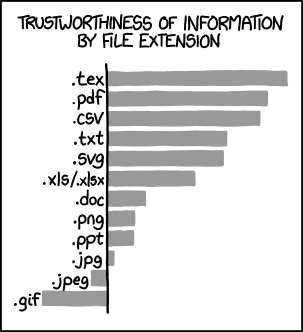
\includegraphics[width=0.4\textwidth]{images/file_extensions.png}
\end{figure}
{\textcolor{white}{\tiny\href{https://xkcd.com/1301/}{https://xkcd.com/1301/}}}
}